%% beamerthemeImperialPoster v1.0 2016/10/01
%% Beamer poster theme created for Imperial College by LianTze Lim (Overleaf)
%% LICENSE: LPPL 1.3
%%
%% This is the example poster demonstrating use
%% of the Imperial College Beamer Poster Theme
\documentclass[xcolor={table}]{beamer}
%% Possible paper sizes: a0, a0b, a1, a2, a3, a4 (although Imperial College posters are usually A0 or A1).
%% Possible orientations: portrait, landscape
%% Font sizes can be changed using the scale option.
\usepackage[size=a0,orientation=portrait,scale=1.55]{beamerposter}
\usepackage{amsmath} 						% Adds mathematical features for equations
\DeclareMathOperator{\Tr}{Tr}				% This is adding in a Trace definition for matrices
\usepackage{bbold}							% Adding in fancy letters for 1 operators etc.
\usepackage{mathtools}						% Adds in text for above/below arrows
\usepackage{physics} 						% Just for absolute values etc.
\usepackage{amssymb}						% For natural numbers symbol
\usepackage{dsfont}                         % for identity double stroke
\usepackage{wrapfig}
\renewcommand{\vec}{\vectorbold}            % if we want to redefine the vector 

\newcommand*{\field}[1]{\mathbb{#1}}%		% Defining the natural numbers
\newcommand*\dif{\mathop{}\!\mathrm{d}}		% Adding additional command for nice looking integration variables dx etc, use like " \dif variable " in integrals 
\newcommand*\bigO{\mathop{}\!\mathcal{O}}   % big O notation
\newcommand\ddfrac[2]{\frac{\displaystyle #1}{\displaystyle #2}}    % for creating bigger fractions that look nicer 

\definecolor{GraphRed}{HTML}{ec1c24}
\definecolor{GraphBlue}{HTML}{00a8f3}
\definecolor{GraphGreen}{HTML}{a1ecb6}

\graphicspath{ {images/} }	

\usetheme{ImperialPoster}

%% Four available colour themes
\usecolortheme{ImperialWhite} % Default
% \usecolortheme{ImperialLightBlue}
% \usecolortheme{ImperialDarkBlue}
% \usecolortheme{ImperialBlack}

\title{CMTH Research}


% \setbeamertemplate{bibliography item}{\insertbiblabel}
% \addbibresource{supersolid.bib}




\begin{document}
\small
\begin{frame}[fragile=singleslide,t]\centering

\maketitle

\begin{columns}[onlytextwidth,T]

%%%% First Column
\begin{column}{.47\textwidth}

\begin{block}{Metamaterials}
Metamaterials are artificial solids designed to guide electromagnetic fields in
ways never seen in nature. Light harvesting techniques can gather radiation from
all directions and concentrate the energy into subwavelength region of a few
cubic nanometres. We can also use a 'trapped rainbow' principle to slow and even
stop light. This opens the door to light localization in time and an innovative
type of cavity-free lasing. 
\end{block}

\begin{figure}
    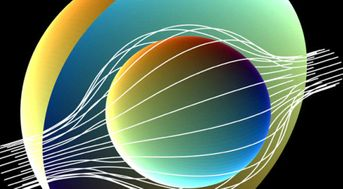
\includegraphics[width=\columnwidth, height=0.15\textheight]{metamaterials.jpg}
    \caption{\footnotesize Stuff}
\end{figure}

\begin{block}{Complexity and Networks}
The richness and complexity in condensed matter physics reflects the
fact that new organised behaviour emerge from the collective behaviour of simple
interacting objects, whether they are electrons in a metal or agents in a social
network. The study of emergent phenomena is a central theme of modern condensed
matter physics. We are part of the Complexity and Networks Group at Imperial
which focus on the interdisciplinary application of these principles to a
variety of stochastic phenomena, ranging from ant colonies to cardiovascular
biology, from sandpiles to earthquakes.
\end{block}

\begin{figure}
    \centering
    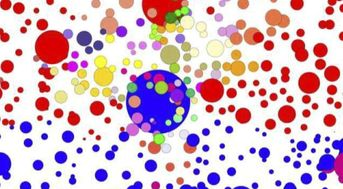
\includegraphics[width=1.\columnwidth, height=0.2\textheight]{complexity.jpg}
    \caption{\footnotesize More things}
\end{figure}

\end{column}

%%%% Second Column
\begin{column}{.47\textwidth}

\begin{block}{Correlated Quantum Systems}
On the microscopic scale, strongly correlated quantum systems exhibit also
emergent phenomena in terms of exotic quantum phases of matter in equilibrium or
novel dynamical behaviour out of equilibrium. Our work encompasses a wide
variety of quantum mechanical systems such as nano-electromechanical devices,
liquid helium films and ultracold atomic clouds.
\end{block}

\begin{figure}
    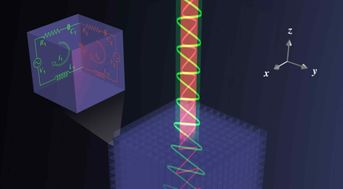
\includegraphics[width=1\columnwidth, height=0.2\textheight]{correlated.jpg}
    \caption{\footnotesize More captions}
\end{figure}

\begin{block}{Simulation of electronic structure}
Our work on materials theory and simulation is linked both to the Centre for
Doctoral Training on the Theory and Simulation of Materials and the London-wide
Thomas Young Centre. New materials have played a central role in the development
of civilisation from the Bronze Age to the Semiconductor Age. We have developed
widely used computational codes to solve the equations of quantum mechanics to
predict the electronic behaviour at the nanoscale, structural properties at the
microscale, or material behaviour on macroscopic length and time scales.
\end{block}

\begin{figure}
    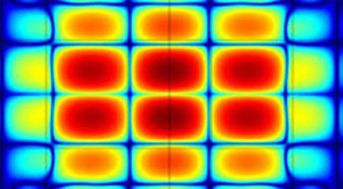
\includegraphics[width=\columnwidth, height=0.15\textheight]{simulation_materials.jpg}
    \caption{\footnotesize Hello}
\end{figure}

\end{column}
\end{columns}

\end{frame}
\end{document}